\chapter{Electromagnetism}

\section{Electrostatics}

\begin{definition}[Electric charge] A scalar quantity that can describe an object. It can be positive or negative
\end{definition}

\begin{definition}[Elementary charge ($e$)] The smallest possible charge $e \approx 1.6 * 10^{-19} \, \Coulomb$.
\end{definition}

\subsection{Charging}

\begin{procedure}[Charging by friction] Rub two nonconductive objects together. The one with the greater electron affinity (electronegativity) becomes negatively charged.
\end{procedure}

\begin{procedure}[Polarization] When two objects near each other, their charge distributions will change in order to ensure that similar charges in the different objects don't get too near each other.
\end{procedure}

% TODO: Conduction and induction

\subsection{Electric fields}

\begin{definition}[Permittivity of free space ($\varepsilon_0$)]
  \[
    \varepsilon_0 \approx 8.85 * 10^{-12} \frac{\Coulomb^2}{\Newton \metre^2}
  \]
\end{definition}

\begin{definition}[Coulomb's constant ($k$)]
  \[
    k = \frac{1}{4\pi\varepsilon_0} \approx 8.99 * 10^9 \, \frac{\Newton \metre^2}{\Coulomb^2}
  \]
\end{definition}

\begin{namedlaw}[Coulomb's Law]
  If stationary point or spherical charges $q_1$ and $q_2$ are near each other but not touching, then the magnitude of the electrostatic force between the two objects is
  \[
    |F_e| = \frac{k |q_1| |q_2|}{r^2} = \frac{|q_1| |q_2|}{4 \pi \varepsilon_0 r^2}
  \]
\end{namedlaw}

\begin{definition}[Electric field]
  The vector field $E$ ($\frac{\Newton}{\Coulomb}$), which applies to all objects.

  The electric field points away from positive charges and towards negative charges.
\end{definition}

\begin{law}
  The electrostatic force on a stationary point or spherical charge $q$ is 
  \[
    F_e = Eq
  \]
  where $E$ is the strength and direction of the electric field.
\end{law}

\begin{law}[by Coulomb's Law]
  The electric field at distance $r$ due to a stationary point or spherical charge $Q$ is
  \[
    E = \frac{kQ}{r^2} = \frac{Q}{4\pi\varepsilon_0 r^2}
  \]

  The electric field at distance $r$ due to a charged object whose total charge is $\int dq$ is
  \[
    E = \int \frac{k \,dq}{r^2} = \int \frac{dq}{4 \pi \varepsilon_0 r^2}
  \]
  where $r$'s tail is at the charge and points towards the point for which we want to calculate $E$.
\end{law}

\begin{definition}[Charge density]
  \begin{align*}
    \text{3D: density} \qquad & \rho = \frac{Q}{v} = \frac{dq}{dV} & (\frac{\Coulomb}{\metre^3}) \\
    \text{2D: surface density} \qquad & \sigma = \frac{Q}{A} = \frac{dq}{dA} & (\frac{\Coulomb}{\metre^2}) \\
    \text{1D: linear density} \qquad & \lambda = \frac{Q}{L} = \frac{dq}{dx} & (\frac{\Coulomb}{\metre}) \\
  \end{align*}
\end{definition}

\begin{example}[E-field of a sheet of charge]
  The magnitude of the E-field caused by a sheet of charge is
  \[
    E = \frac{\sigma}{2\varepsilon_0}
  \]
  where the E-field points away from the sheet if the charge is positive, and towards the sheet if the charge is negative.
\end{example}

\begin{example}[E-field of a cylindrical charge]
  The magnitude of the E-field caused by a cylindrical charge of radius $R$ with negligible end effects, at radius $r$ from its axis, is:
  \[
    \frac{R\sigma}{r\varepsilon_0}
  \]
\end{example}

\subsection{Electric flux}

\begin{definition}[Electric flux ($\Phi$)]
  The flux through a surface with area vector $\vec{A}$ is
  \[
    \Phi_E = \int \vec{E} \dotp d\vec{A} \qquad \left(\frac{\Newton \metre^2}{\Coulomb}\right)
  \]
  where $\vec{E}$ is the electric field that passes through the surface, and the area vector's magnitude is the area and direction is normal/perpendicular to the surface.
\end{definition}

\begin{definition}[Net flux]
  The flux through any surface that encloses a charge.
\end{definition}

\begin{namedtheorem}[Gauss's Law]
  The net flux is equivalent to the enclosed charge divided by the permittivity of free space, and can be equated to the flux through the surface:
  \[
    \Phi_{\text{net}} = \frac{q}{\varepsilon_0} = 4\pi k q = \oint \vec{E} \dotp d\vec{A}
  \]
\end{namedtheorem}

\subsection{Electric potential}

\begin{definition}[Electric potential energy]
  The work required to move a charge from a reference position to its current location in the electric field.

  When the electrostatic force does work $W_e$ on the object, its electric potential energy decreases and its kinetic energy increases:
  \[
    \Delta U_e = -W_e
  \]
\end{definition}

\begin{definition}[Electric potential]
  The work per unit charge required to move a charge from a reference position to its current location in the electric field.
\end{definition}

\begin{definition}[Electric potential difference / Voltage]
  The difference in electric potential between two points.

  \[
    \Delta V = \frac{\Delta U_e}{q} = -\frac{W_e}{q} = -\int \vec{E}(\vec{r}) \dotp d\vec{r} 
  \]

  Therefore,
  \[
    \vec{E} = - \frac{dV}{dr}
  \]
\end{definition}

\begin{lemma}
  If an electric potential $V$ between two points separated by distance $L$ is caused by a uniform electric field of strength $E$,
  \[
    V = -EL
  \]
\end{lemma}

\begin{definition}[Equipotential line/surface]
  A line/surface where for each point on the line/surface, the electric potential is the same.
  
  Graphs of equipotential lines where each line's electric potential is an integer multiple of some number produce a topographic-like map of the electric field, where each of the equipotential lines can be viewed as contour lines.
\end{definition}

\begin{theorem}[Potential caused by a point or spherical charge]
  The electric potential outside a point or spherical charge, at distance $r$ from the center of the charge, is
  \[
    \frac{kq}{r}
  \]

  The electric potential inside a spherical charge of radius $R$ is
  \[
    \frac{kq}{R}
  \]

  (This derives from Coulomb's Law.)
\end{theorem}

\section{Circuits}

\subsection{Capacitance}

\begin{definition}[Capacitor]
  At least one charged conductor, usually two.

  Common capacitor shapes:
  \begin{itemize}
    \item Parallel plate
    \item Cylindrical
    \item Spherical
  \end{itemize}

  The symbol for a capacitor is
  \begin{circuitikz}
    \draw (0,0) to [capacitor] (5,0); 
  \end{circuitikz}
\end{definition}

\begin{definition}[Capacitance]
  Where $Q$ is the magnitude of the charge on one of the plates, and $V$ is the potential difference between two plates:

  \[
    C = \frac{Q}{V} \qquad \left(\Farad = \frac{\Coulomb}{\Volt}\right)
  \]

  The capacitance remains constant for a given capacitor regardless of any change in charge or voltage; it only depends on the shape of the capacitor.

  The capacitance is a positive (unsigned) value.
\end{definition}

\begin{example}[Parallel plate capacitor]
  The capacitance of a capacitor containing two parallel plates, where each plate has area $A$ and the distance between the plates is $d$, is
  \[
    C = \frac{\varepsilon_0 A}{d}
  \]
\end{example}

\begin{example}[Spherical shell capacitor]
  The capacitance of a capacitor containing two concentric spherical shells, where the smaller shell has radius $a$ and the larger has radius $b$, is
  \[
    C = \frac{ab}{bk - ak}
  \]
\end{example}

\begin{example}[Cylindrical capacitor]
  The capacitance of a capacitor containing two concentric cylindrical shells with negligible end effects, where the smaller shell has radius $a$ and the larger has radius $b$ and both have length $L$, is
  \[
    C = \frac{2 \pi \varepsilon_0 L}{\ln\left(\frac{b}{a}\right)}
  \]
\end{example}

\begin{theorem}[Energy stored in a capacitor]
  \[
    U_e = \frac{1}{2} \frac{Q^2}{C} = \frac{1}{2} VQ = \frac{1}{2} C V^2
  \]
\end{theorem}

\begin{definition}[Dielectric]
  An object that can be polarized.
\end{definition}

\begin{definition}[Permittivity]
  The permittivity of space containing a dielectric is equal to
  \[
    K\varepsilon_0
  \]
  where $K$ is the dielectric's \textbf{dielectric constant}.
\end{definition}

\subsection{Miscellaneous circuit stuff}

\begin{definition}[Battery]
  A battery has two terminals, a positive and a negative terminal. The positive terminal has higher electric potential than the negative terminal, and the battery creates an E-field between the positive and negative terminal. The potential difference between the positive and negative terminal is called the \textbf{voltage} of the battery, and is represented as $\mathcal{E}$.

  The electric field causes positive current to flow from the positive to negative terminal. Equivalently, negative current flows from the negative to positive terminal, which is the way the actual electrons flow.

  The symbol for a battery is
  \begin{circuitikz}
    \draw (0,0) to [battery1=$\,$] (5,0); 
  \end{circuitikz}
\end{definition}

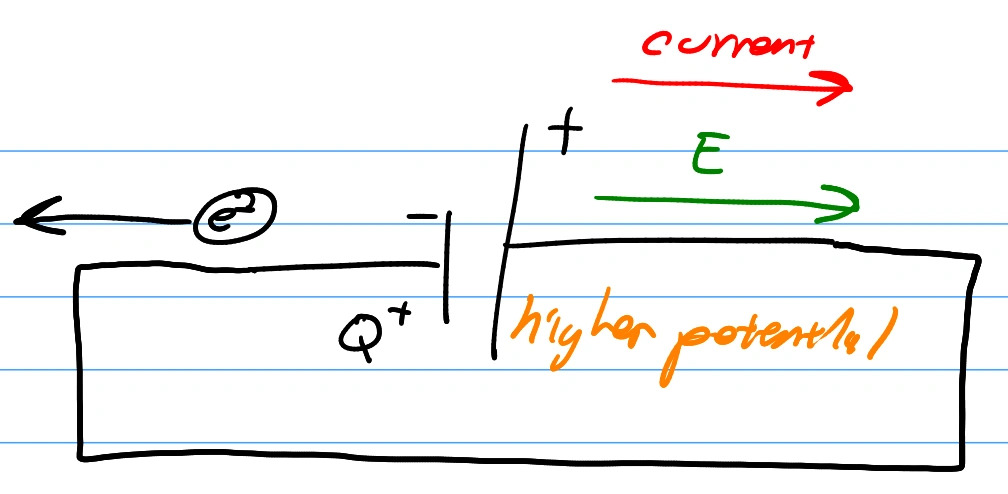
\includegraphics[width=8cm]{content/electromagnetism/battery-simple-circuit.jpg}

\subsection{Loop Law}

\begin{namedlaw}[Loop Law]
  In a circuit, the sum of the signed potential differences along the entire circuit is 0.

  \[
    \sum \Delta V = 0
  \]

  In a circuit with a battery, this means that the voltage (unsigned) of the battery is equal to the sum of the other potential differences along the circuit.
\end{namedlaw}

If a set of capacitors were replaced by a single capacitor without changing any of the observable properties of the circuit, then $C_\text{eq}$ (the \textbf{equivalent capacitance}) is equal to the capacitance of that single capcitor and $Q_\text{eq}$ (the \textbf{equivalent charge}) is equal to the capacitance of one plate of that single capacitor.

\begin{example}[Capacitors in parallel]
  \begin{align*}
    C_\text{eq} &= \sum C_i \\
    \mathcal{E} &= V_1 = \cdots = V_n \\
    Q_\text{eq} &= \sum Q_i
  \end{align*}
\end{example}

\begin{example}[Capacitors in series]
  \begin{align*}
    \frac{1}{C_\text{eq}} &= \sum \frac{1}{C_i} \\
    \mathcal{E} &= \sum V_i \\
    Q_\text{eq} &= Q_1 = \cdots = Q_n
  \end{align*}
\end{example}

\subsection{Current and resistance}

\begin{definition}[Current / amperage ($i$ or $I$)]
  The rate at which charges flow through a conductor.

  \[
    i = I = \frac{dq}{dt} \qquad \left(\Ampere = \frac{\Coulomb}{\second}\right)
  \]
\end{definition}

\begin{definition}[Junction]
  A place in a circuit at which the current can change.
\end{definition}

\begin{law}[Junction Rule]
  The sum of the current into a junction equals the sum of the current out of the junction.
  \[
    \sum I_\text{into} = \sum I_\text{out}
  \]
\end{law}

\begin{definition}[Current density]
  \[
    J = \frac{i}{A}
  \]
\end{definition}

\begin{definition}[Resistance ($R$)]
  \[
    R = \frac{V}{i} \qquad \left( \Ohm = \frac{\Volt}{\Ampere} \right)
  \]

  The resistance is a property of the conducting object.
\end{definition}

\begin{namedlaw}[Ohm's Law]
  \[
    V = iR
  \]
\end{namedlaw}

\begin{definition}[Resistivity]
  \[
    \rho = \frac{E}{J} \qquad \left( \Ohm \metre \right)
  \]

  The resistivity is a property of the conducting material.
\end{definition}

\begin{lemma}
  The resistance of a uniform conductor of length $L$, cross-sectional area $A$, and resistivity $\rho$ is
  \[
    R = \frac{\rho L}{A}
  \]
\end{lemma}

\begin{law}
  \[
    Q = Nq
  \]
  where $N$ is the number of charge carriers and $q$ is the charge of each charge carrier.

  If the charge carrier is an electron (as usual), then
  \[
    Q = Ne
  \]
\end{law}

\begin{definition}[Drift speed]
  \[
    v_\text{drift} = \frac{J}{nq}
  \]
  where $n = \frac{N}{\text{Volume}}$ (the charge carrier density), and $q$ is the charge of each charge carrier ($q = e$ if the charge carrier is an electron).
\end{definition}

\begin{theorem}[Power consumed by a resistor]
  Most of this energy is converted to heat.
  \[
    P = IV = I^2 R = \frac{V^2}{R}
  \]
\end{theorem}

\begin{lemma}[Resistors in parallel]
  By the Loop Law,
  \[
    V_{eq} = V_1 = \cdots = V_n
  \]

  By the Junction Rule,
  \[
    \frac{\mathcal{E}}{R_{eq}} = i_{\text{total}} = \sum i_i
  \]

  Therefore by Ohm's Law,
  \[
    \frac{1}{R_{eq}} = \sum \frac{1}{R_i}
  \]
\end{lemma}

\begin{lemma}[Resistors in series]
  By the Loop Law,
  \[
    V_{eq} = \sum V_i
  \]

  Therefore by Ohm's Law,
  \[
    R_{eq} = \sum R_i
  \]
\end{lemma}

\subsection{RC circuits}

\begin{definition}[RC circuit]
  A circuit with a resistor and a capacitor.
\end{definition}

\begin{definition}[Time constant]
  For an RC circuit,
  \[
    \tau := R_{eq} C_{eq} \qquad (\second)
  \]
\end{definition}

\begin{law}[Charging a capacitor]
  A capacitor can be charged by applying an $\mathcal{EMF}$ such as a battery on both sides of the capacitor, possibly including a resistor or resistors with equivalent resistance $R$.

  Initial and final conditions:
  \begin{align*}
    t &= 0 & t &\to \infty \\
    q_0 &= 0 & q_{\text{max}} &= C\mathcal{E} \\
    i_0 &= \frac{\mathcal{E}}{R} & i_f &= 0 \\
  \end{align*}

  Applying the loop law:
  \[
    \mathcal{E} - R \frac{dq}{dt} - \frac{q}{c} = 0
  \]

  Solving the equation, we get:
  \begin{align*}
    q(t) &= q_{\text{max}} \left(1 - e^{- \frac{t}{\tau}}\right) \\
    i(t) &= i_0 e^{- \frac{t}{\tau}}
  \end{align*}
\end{law}

\begin{law}[Discharging a capacitor]
  A capacitor can be discharged by shorting both plates, possibly including a resistor or resistors with equivalent resistance $R$ in between.

  Initial and final conditions:
  \begin{align*}
    t &= 0 & t &\to \infty \\
    q_{\text{max}} &= C\mathcal{E} & q_f &= 0 \\
    i_0 &= -\frac{\mathcal{E}}{R} & i_f &= 0 \\
  \end{align*}

  Applying the loop law:
  \[
    - R \frac{dq}{dt} - \frac{q}{c} = 0
  \]

  Solving the equation, we get:
  \begin{align*}
    q(t) &= q_{\text{max}} e^{- \frac{t}{\tau}} \\
    i(t) &= i_0 e^{- \frac{t}{\tau}}
  \end{align*}

  (ensure $i_0 < 0$)
\end{law}

\subsection{Magnetism}

\begin{definition}[Magnetic field ($\vec{B}$)]
  The field lines exit through the north pole of the magnet and enter through the south pole of the magnet. They always form a closed loop.

  A magnetic field is caused by a moving charged particle, and is perpendicular to the velocity of a particle, as described by the right hand rule - if the velocity $\vec{v}$ is represented by the right-hand thumb, then curling the rest of the fingers will give the direction of the $\vec{B}$-field.
\end{definition}

\begin{definition}[Permanent magnet]
  A magnet (north and south pole) which stays magnetic without a current or other external force being applied.

  It is caused when the electron spins within the magnet are all aligned.
\end{definition}

\begin{definition}[Solenoid]
  A coiled conducting wire.

  If a current is run through the solenoid, it becomes an \textbf{electromagnet}.
\end{definition}

\begin{definition}[Magnetic force]
  \[
    \vec{F}_B = q \vec{v} \crossp \vec{B}
  \]
  therefore
  \[
    |F_B| = q |v| |B| \sin \theta
  \]
\end{definition}

\begin{lemma}[Magnetic force on a straight wire]
  Given a wire of length $l$ (define $\vec{l}$ to be the vector whose magnitude is the length of the wire and whose direction is the direction of the current), with current $i$ passing through it, in a uniform external magnetic field $\vec{B}_{\text{ext}}$,
  \[
    \vec{F}_B = i \vec{l} \crossp \vec{B}_{\text{ext}}
  \]
\end{lemma}

\begin{definition}[Permeability of free space]
  \[
    \mu_0 = 4\pi * 10^{-7} \qquad \frac{\Tesla \metre^2}{\Ampere}
  \]
\end{definition}

\begin{namedlaw}[Biot-Savart Law]
  The B-field at point $P$ caused by a point current part of a longer current-carrying object is
  \[
    d\vec{B} = \frac{\mu_0 i}{4 \pi} \frac{d\vec{s} \crossp \hat{r}}{r^2}
  \]
  where $d\vec{s}$ is the length of the point current and $\hat{r}$ is the unit vector of the vector from the point current to $P$.
\end{namedlaw}

\begin{namedlaw}[Ampère's Law]
  The B-field along an Amperian loop (a closed loop) is related to the enclosed current by
  \[
    \oint \vec{B} \dotp d\vec{s} = \mu_0 i_{\text{enc}}
  \]

  where $d\vec{s}$ represents the length of a infinitesimally small segment of the Amperian loop and $i_{\text{enc}}$ represents the current enclosed by the Amperian loop. ($\vec{B}$ is measured at each point along the Amperian loop.)
\end{namedlaw}

\begin{example}[B-field due to a straight wire]
  The B-field due to a straight wire carrying current $i$, measured at a distance $r$ from the center of the wire, is
  \[
    B = \frac{\mu_0 i}{2 \pi r}
  \]

  Within the straight wire with a radius of $R$, at a distance $r$ from the center of the wire,
  \[
    B = \frac{\mu_0 i r}{2 \pi R^2}
  \]
\end{example}

\begin{example}[B-field inside a solenoid]
  The B-field along the central axis inside a solenoid with $n$ loops of wire per unit length carrying current $i$, is
  \[
    B_0 = \mu_0 n i
  \]
\end{example}

\subsection{Magnetic flux}

\begin{definition}[Magnetic flux]
  The flux through a surface with area vector $\vec{A}$ is
  \[
    \Phi_B = \int \vec{B} \dotp d\vec{A} \qquad \left(\Weber = \Tesla \metre^2\right)
  \]
  where $\vec{B}$ is the $B$-field that passes through the surface, and the area vector's magnitude is the area and direction is normal/perpendicular to the surface.
\end{definition}

\begin{namedlaw}[Faraday's Law]
  The emf induced by a changing magnetic flux through the surface through a closed conductive loop is
  \[
    \mathcal{E} = - N \frac{d\Phi_B}{dt}
  \]
\end{namedlaw}

\begin{namedlaw}[Lenz's Law]
  The direction of the induced emf (and thus the induced current) is such that the induced magnetic field it produces opposes the change in the magnetic flux that caused it.
\end{namedlaw}

\begin{theorem}[by Lenz's Law]
  An increasing magnetic flux induces a $B$-field in the opposite direction of the changing flux.

  An decreasing magnetic flux induces a $B$-field in the same direction as the changing flux.

  The induced current's direction is determined by the induced $B$-field using the right-hand rule.
\end{theorem}

\subsection{Inductors}

\begin{definition}
  A device which stores energy in a magnetic field, based on the current flowing through it.
\end{definition}

\begin{definition}[Inductance]
  The inductance of an inductor with $N$ loops, with current $I$ flowing through it, and where $\Phi_B$ is the flux through the surface bounded by one loop of the inductor:
  \[
    L = \frac{N \Phi_B}{I} \qquad \left( \Henry \frac{\Tesla \metre^2}{\Ampere} \right)
  \]
\end{definition}

\begin{theorem}[Inductance of a solenoidal inductor]
  The inductance of a solenoid with $n$ loops of wire per unit length, of length $l$, where $A$ is the area of the surface bounded by one loop of the solenoid, is
  \[
    L = \mu_0 n^2 A l
  \]
\end{theorem}

\begin{theorem}[Constitutive equation]
  The EMF induced by an inductor is given by 
  \[
    \mathcal{E} = - L \frac{di}{dt}
  \]

  The direction is specified by Lenz's Law.
\end{theorem}

\begin{theorem}[Energy stored in an inductor]
  The energy stored in an inductor is
  \[
    U_L = \frac{1}{2} LI^2
  \]
\end{theorem}

\subsection{RL circuits}

\begin{definition}[RL circuit]
  A circuit with a resistor and an inductor.
\end{definition}

\begin{definition}[Inductive time constant]
  For an RL circuit,
  \[
    \tau_L := \frac{L}{R} \qquad (\second)
  \]
\end{definition}

\begin{theorem}[Behavior of an RL circuit with a battery]
  By the Loop Law,
  \[
    \mathcal{E} - IR - L \frac{di}{dt} = 0
  \]

  Solving the diffeq, we get
  \[
    I(t) = \frac{\mathcal{E}}{R} \left(1 - e^{- \frac{t}{\tau_L}}\right)
  \]

  The circuit starts off with no current, and as time goes on the current increases until it reaches its final value $I = \frac{\mathcal{E}}{R}$ at which point the inductor stores its max energy.
\end{theorem}

\begin{theorem}[Behavior of an RL circuit after the battery is disconnected]
  By the Loop Law,
  \[
    - IR - L \frac{di}{dt} = 0
  \]

  Solving the diffeq, we get
  \[
    I(t) = \frac{\mathcal{E}}{R} e^{- \frac{t}{\tau_L}}
  \]

  The circuit starts off with current of $I = \frac{\mathcal{E}}{R}$ and ends with no current, at which point the inductor stores no energy.
\end{theorem}

\subsection{LC circuits}

\begin{definition}[LC circuit]
  A circuit with an inductor and a capacitor.

  This circuit stores energy. At some times the capacitor stores energy, but the capacitor discharges into the inductor until the inductor stores all the energy. Then the inductor releases energy towards the capacitor, causing the capacitor to store all the energy but with the positive and negative side swapped.
\end{definition}

\begin{theorem}
  \[
    \omega = \frac{1}{\sqrt{LC}} \qquad f = \frac{1}{2\pi \sqrt{LC}}
  \]

  The charge and current on one plate of the capacitor is given by
  \[
    q(t) = Q \cos(\omega t) \qquad i(t) = q'(t) = -Q \omega \sin(\omega t)
  \]

  where $Q$ is the maximum charge on one plate of the capacitor.

  The energy in the LC circuit is:
  \[
    U_{\text{total}} = \frac{1}{2} \frac{Q^2}{C} = U_e + U_L = \frac{1}{2} \frac{q^2}{C} + \frac{1}{2} Li^2
  \]
\end{theorem}
